\documentclass[14pt,a4paper]{extarticle}
\usepackage[a4paper,margin=20mm]{geometry}
\usepackage[french]{babel}
\usepackage[french]{babel}
\frenchbsetup{StandardLists=true} % à inclure si on utilise \usepackage[french]{babel}
\usepackage{enumitem}
\usepackage[utf8]{inputenc}
\usepackage[T1]{fontenc}
\usepackage{lmodern}
\usepackage{amsmath}
\usepackage{amssymb}
\usepackage{mathrsfs}
\usepackage{fancybox}
\usepackage{graphicx}
\usepackage{wrapfig}
\usepackage{textcomp}
\usepackage{xcolor}
\usepackage{listings}
\newcommand{\ud}{\mathrm{d}}
\newcommand{\hsp}{\hspace{20pt}}
\newcommand{\HRule}{\rule{\linewidth}{0.5mm}}
\newcommand{\fouine}{\textsc{Fouine }}

\begin{document}

%\maketitle
\begin{titlepage}
    \begin{sffamily}
        \begin{center}


            \textsc{\LARGE École Normale Supérieure de Lyon}\\[3cm]

            \textsc{\Large Rapport de Projet}\\[2.5cm]

            \HRule \\[0.4cm]
            \textsc{\huge Présentation de notre interpréteur de notre language Fouine}
            \HRule \\[3cm]

            \begin{minipage}[c]{.46\linewidth}
                \centering
                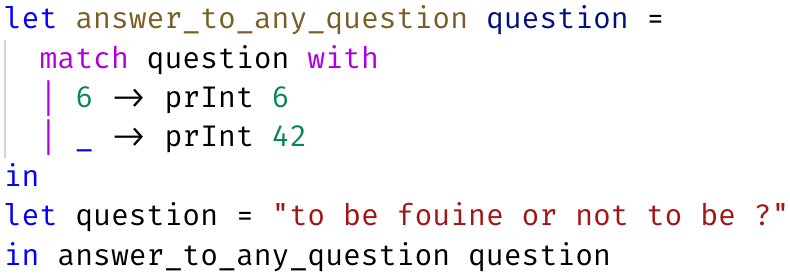
\includegraphics[width=7cm]{fouine short example.png}
            \end{minipage}
            \hfill%
            \begin{minipage}[c]{.46\linewidth}
                \centering
                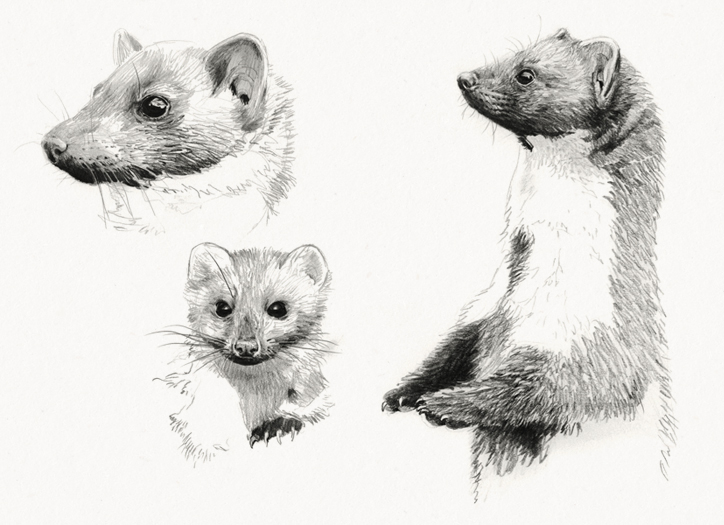
\includegraphics[width=7cm]{20_martes-foina.jpg}
            \end{minipage}\\[3cm]
            % Author and supervisor
            \hspace{-0.8cm}
            \begin{minipage}{0.4\textwidth}
                \begin{flushleft} \large
                    Maxime \textsc{Cautrès}\\
                    Pierre \textsc{Goutagny}\\
                \end{flushleft}
            \end{minipage}
            \hspace{3cm}
            \begin{minipage}{0.4\textwidth}
                \begin{flushright} \large
                    \emph{Encadrant :} \\
                    Daniel \textsc{HIRSCHKOFF}\\
                \end{flushright}
            \end{minipage}

            \vfill

            % Bottom of the page
            {\large  Janvier 2021 - Mai 2021}
        \end{center}
    \end{sffamily}
\end{titlepage}

\newpage

\newpage

\section{Organisation}

\subsection{Le travail à deux}

\paragraph{Répartition}
Le projet \fouine  se faisant à deux, nous avons du
apprendre à nous organiser pour partager le travail.
La structure globale des rendus, demandant l'implémentation
de fonctionalités étapes par étapes aidait quant à la
répartitions des tâches. Cependant, principalement lors
du début des premiers rendus, il était difficile de
séparer les premières tâches car elles était très proches.
Cela nous a obligé à travailler ensemble pendant un petit
temps avant que nous puissions travailler de manière indépendante.

\paragraph{Entraide}
Le fait d'être à deux pour un projet comme celui-ci nous a
beaucoup plu. Effectivement, si l'un de nous bloquait sur
un point précis, il pouvait aller demander de l'aide ou son
avis à l'autre, sa compréhension ou un détail de l'implémentation.
Cela a permis de grandement accélérer le processus de développement
du projet et aussi la qualité des rendus.

\subsection{Git}

\paragraph{Le gestionaire de version}
Le fait que Git permette de remonter dans le
temps a été essentiel. Malgré la réflexion sur papier
avant de commencer à coder, il y a eu de nombreux faux
départs. Le gestionnaire de version nous a facilement
permis de revenir en arrière pour recommencer à travailler
à partir d'une base solide.\\[1cm]

\hspace{-0.75cm}
\begin{minipage}[c]{0.5\linewidth}
    \paragraph{Les branches}
    Elles ont joué un rôle crucial dans l'organisation de notre
    travail. Lorsque les tâches à implémenter étaient assez
    indépendentes, nous créions une branche par tâche en cours. Cela
    nous à donner un \textit{work flow} très \textit{efficient}. La branche master était
    toujours fonctionnelle, lorsque l'on commençait une tâche, on partait
    de master, faisions l'implémentation dans la branche, rajoutions les
    tests puis une fois que tout marchait nous mergions à nouveaux avec
    master. Cela nous à permis de travailler de manière indépendante sur
    des mêmes zones du code sans avoir à continuellement gérer des merge
    conflicts.


\end{minipage}
\hfill%
\begin{minipage}[c]{.46\linewidth}
    \centering
    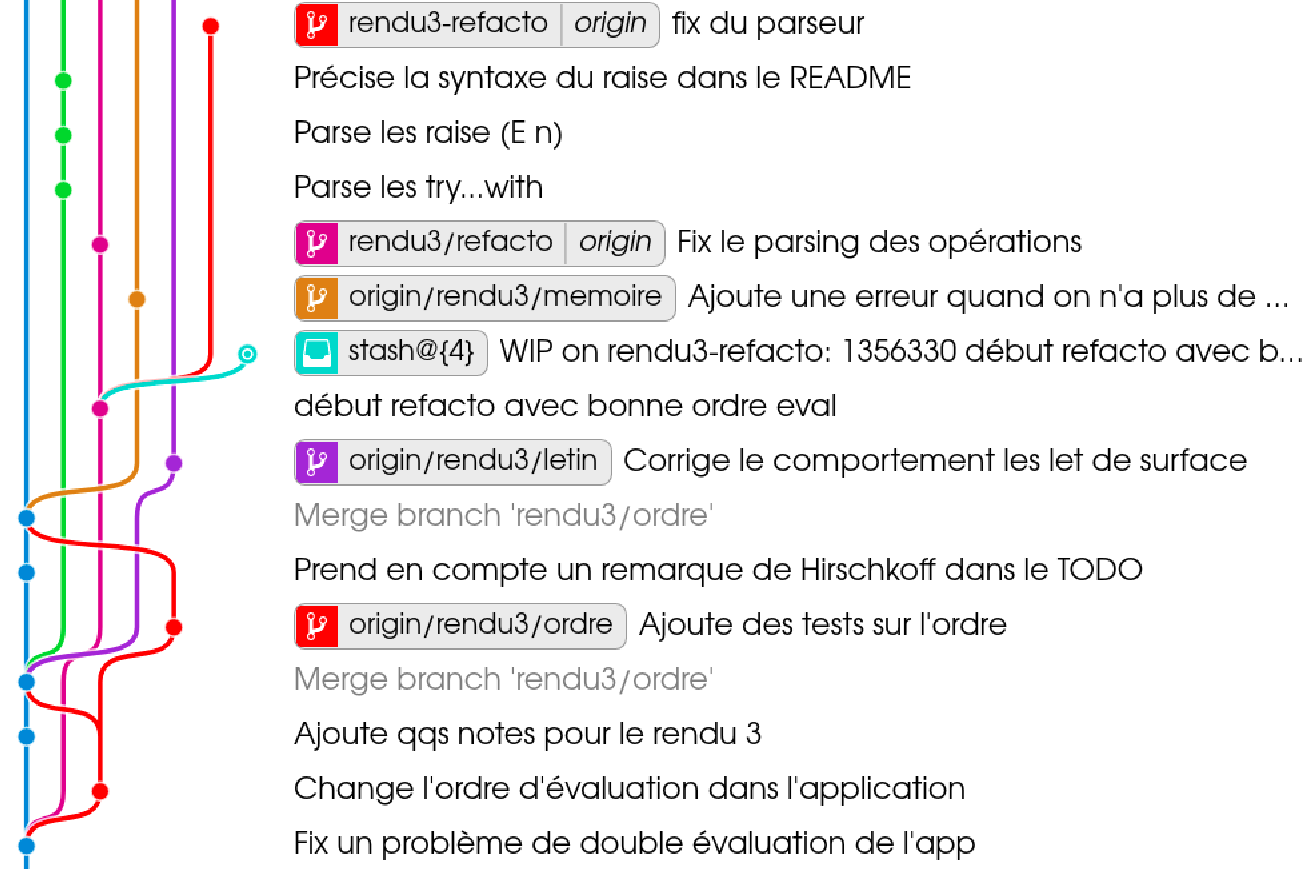
\includegraphics[height=6cm]{git_branching.png}
\end{minipage}\\[1cm]


\paragraph{Ce que Git nous à apporté}
Pour conclure sur l'utilisation de git, ce projet nous a poussé
à approfondir nos connaissances sur le fonctionnement de git, les
branches, la gestions des versions et autres. Cela nous sera fortement
utile dans le futur et directement dans le futur proche avec le projet intégré du
M1 où l'utilisation de git sera primordiale à l'hygiène du projet.

\subsection{Les tests}

\paragraph{Le maitre mot: Unitaire}
Lors de se projet il y avait énormement de choses à implémenter.
Pour être sur qu'a chaque étape ce que nous faisions était fonctionnel,
nous avons ajouté une importante quantité de tests unitaires, ces tests
ont pour but de valider la fonctionnalité venant d'être ajouté, mais aussi
de vérifier que l'ajout de la fonctionalité n'a pas cassé d'autres déjà
existante. Le fait de les rendre unitaire permettait de très rapidement
identifier les problèmes si il y en avait pour mieux les traiter.

\paragraph{Des tests plus généraux}
Tout ces tests unitaires ont été complété à la fin de chaque rendu par des tests
plus important qui servait alors de démonstration/examples de ce que notre \fouine
savait faire. Il avait aussi pour but de vérifier que les fonctionalités toutes mises
ensemble fonctionnaient toujours.

\section{Fouine}

\subsection{Le parsing}

\paragraph{Ocaml yacc}
Pour le parsing nous avons décidé de rester sur Ocaml yacc car
nous commencions à bien parser \fouine. Nous avons fait évoluer la manière
dont nous parsions au fur et à mesure du projet pour l'adapter aux factorisations
de code. Nous avons tout les deux manipulé le parseur lors de différentes phases des rendus.

\subsection{L'évaluation}

\paragraph{L'évaluation}
Pour l'évaluation, il n'y a pas grand chose a signaler, l'implémentationde ce qui était
demandé s'est bien déroulé et il n'y a guère eu de choix important à mettre en place. Les
difficultés était concentrées autour des matchings et des motifs.

\paragraph{La continuation}
Pour le rendu 3 il était demandé de modifier l'évaluation pour
quelle fonctionne par continution. Cela a permis de parser et
evaluer les exceptions, sans utiliser les exceptions d'ocaml.
La seconde partie du rendu 3 ce chargeait de la traduction en
CPS, cela fut plus technique que nous le pensions, mais avec
du temps passé sur papier nous avons réussi à obtenir une traduction
cps presque agréable à lire \cite{HIRSCHKOFF}

\subsection{Le typage}
Le typage s'est plutôt bien passé, nous avons pris notre temps
pour faire les choses bien et de manière efficace. L'ajout du polymorphisme
a été fais en ajoutant le schéma de typage. Il a été optimisé pour utiliser
le plus de fonctions déjà écrites.

\subsection{Conlusion}
Notre \fouine est capable de faire tout ce qui a été demandé
dans l'ensemble des rendus, mise à part le rectypes que nous
n'avons pas implémenté. Nous sommes satisfait du résultat, ce
projet nous à poussé à faire du code correct ansi que lisible, ce
qui sans aucun doute nous servira plus tard. Ce même code qui de
ce fait est facilement modifiable à rendu le travail sur la fin
très plaisant. Ce projet nous a de plus fait découvir une multitude
de points très subtils voire rageants  d'Ocaml, ce qui nous permet de mieux apprécier
celui-ci. Un article très intéressant \cite{DBLP:journals/cacm/Landin66},
permettrait d'approfondir ce projet.\\[2cm]

Fouinement Vôtres\ldots

\bibliographystyle{plain}
\bibliography{biblio}

\end{document}
